\chapter{The Algorithm}

\section{Reference transformation}

The first step of the algorithm lies in transforming a reference sequence covering the selected active region into a De Bruin-like graph. The idea behind this step is very similar to other assembly algorithms based on De Bruin graphs. 

The reference is divided into k-mers, each overlaps with the adjacent ones by k-1 bases. K-mers representing the same sequence are differentiated by their context number, so each k-mer derived from the reference is unique. Two extra k-mers, denoting the beginning and te end of the active region are added to the set. Then, each k-mer is represented by a single vertex in the graph, and edges are defined by the order of the k-mers within the active region.

Formaly speaking, with the active region of length $l$ as represented as a sequence of bases $(b_0, ..., b_{l-1})$, k-mers $K_0, ..., K_{l-k+2}$ are derived from the region as follows:
\begin{itemize}
\item $K_0 = ((B, b_0, ..., b_{k-2}), 0)$
\item $K_1 = ((b_0, ..., b_{k-1}), 0)$
\item . . .
\item $K_i = ((b_i, ..., b_{i+k-1}), c_i), 2 <= i <=  l-k+1$
\item . . .
\item $K_{l-k+2} = ((b_{l-2k+3}, ..., b_{l-k+1}, E), 0)$
\end{itemize}
$c_i$ represents the context number of the k-mer $K_i$. The number is set to zero for k-mers the sequence of which do not repeat within the active region. On the other hand, let's assume that k-mers $K_{i_0}, ..., K_{i_{n-1}}, i_0 < ... < i_{n-1}$ represent the same sequence. Their context number is defined as
$$
c_{i_j} = j, 
$$

$K_0$ and $K_{l-k+2}$ are special k-mers added to the set in order to show the start and end of the active region within the graph. $B$ and $E$ are virtual bases that ensures these k-mers represent unique sekquences. The bases must not appear in the active region.

After their derivation, each k-mer $K_i$ is transformed into a single vertex $v_i$. Edges follow the order the k-mers occurrs within the active region. In other words, the edge set of the graph is
$$
E = {(v_i, v_{i+1})}, 0 <= i <= l-k+1
$$

Figure \ref{fig:ref-my} displays a graph created by transformation of an active region \texttt{ATCTGTATATATG} with k-mer size of 5. The algorithm derives the following k-mers:
$$
k_0 = ((B, A, T, C, T), 0)
k_1 = ((A, T, C, T, G), 0)
k_2 = ((T, C, T, G, T), 0)
k_3 = ((C, T, G, T, A), 0)
k_4 = ((T, G, T, A, T), 0)
k_5 = ((G, T, A, T, A), 0)
k_6 = ((T, A, T, A, T), 0)
k_7 = ((A, T, A, T, A), 0)
k_8 = ((T, A, T, A, T), 1)
k_9 = ((A, T, A, T, G), 0)
k_{10} = ((T, A, T, G, E), 0)
$$

As can bee seen, there are two k-mers representing sequence \texttt{TATAT}, namely $K_6$ and $K_8$. Because of their distinct context number, their are represented by separate vertices. Introduction of the numbers removed a loop from the graph. The loop can be observed on Figure \ref{fig:ref-db} that shows a classical De Bruin graph constructed from the same active region. K-mers $K_6$ and $K_8$ are represented by the same vertex. In order to recover the sequence, it is required to know how many times the loop was actually used during the transformation step.

\begin{figure}
	\centering
	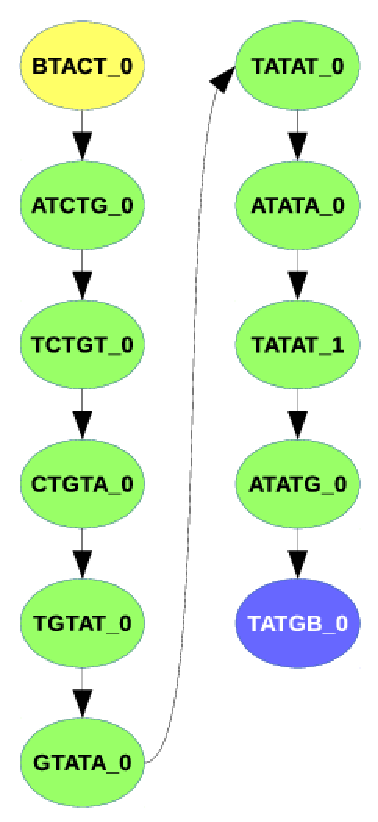
\includegraphics{img/ref-my.pdf}
	\caption{Graph resulting from the transformation of \texttt{ATCTGTATATATG} sequence}
	\label{fig:ref-my}
\end{figure}

\begin{figure}
	\centering
	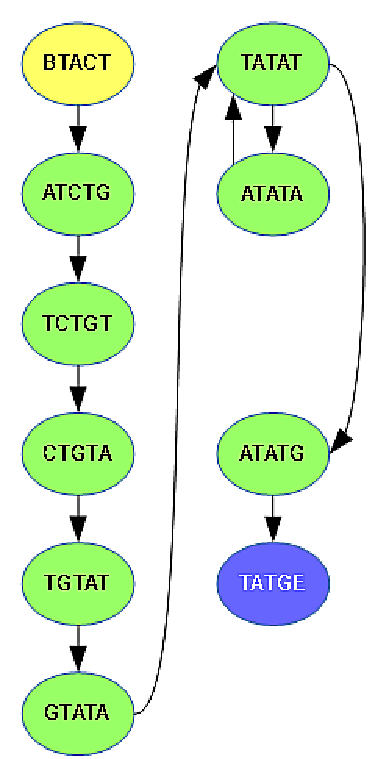
\includegraphics{img/ref-db.pdf}
	\caption{Transformation of the ATCTGTATATATG squence to a standard De Bruin graph (with no k-mer context numbers)}
	\label{fig:ref-db}
\end{figure}

Although we solved the loop problem, for now, by not allowing them to appear, and thus making the graph, at this stage, linear, things get more complicated in the next step that covers introducing individual reads into the graph.

\section{Adding Reads}

Basic idea behind this step is farily simple and similar to the approach used in the previous one. The read being added is divided into a sequence of k-mers. If a k-mer is not represented by any existing graph vertex, a new vertex is created for it. In other cases, existing vertices are used. Again, vertices representing adjacent k-mers in the read are connected by edges. 

\subsection{The Idea}

Figure \ref{fig:read-idea} shows a graph created by transforming a region of \texttt{ACCGTGGTAAT} and adding a read \texttt{ACCGTAGTAAT} to the resulting graph. The read is divided into the following k-mers
$$
k_0 = ((A, C, C, G, T), 0)
k_1 = ((C, C, G, T, A), 0)
k_2 = ((C, G, T, A, G), 0)
k_3 = ((G, T, A, G, T), 0)
k_4 = (T, A, G, T, A), 0)
k_5 = ((A, G, T, A, A), 0)
k_6 = ((G, T, A, A, T), 0)
$$

In the graph, there already are vertices representing k-mers $k_0$ and $k_6$. For other others, new vertices are created. Finally, edges are added (if necessary) to show the k-mers order within the read.

\begin{figure}
	\centering
	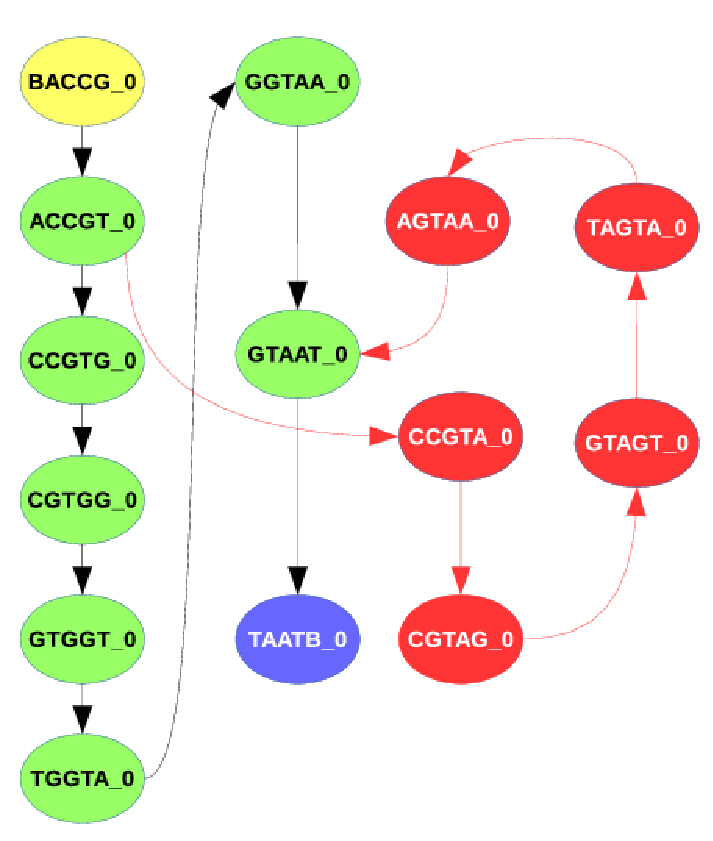
\includegraphics{img/read-idea.pdf}
	\caption{Basic idea behind adding a read into a De Bruin graph}
	\label{fig:read-idea}
\end{figure}

Unfortunately, this idea does not work in our case. Introduction of the k-mer context numbers prevented loops in the graph derived from the reference. But since multiple k-mers representing the same sequence may exist, it is not always possible to easily determine which of the vertices should be assigned to individual k-mers of the read. For example, if looking at the graph from Figure \ref{fig:ref-my}, it is not clear which vertex (or vertices) should be assigned to a k-mer with \texttt{TATAT} sequence. 

\subsection{The Idea Modified}

To solve this issue, we decided to complicate the basic idea a little. The read, defined as a nucleotide sequence $(r_0, ..., r_{m-1}) is still divided into k-mers k_{i} = ((r_i, ..., r_i+k-1), 0)$, 0 <= i <= m-k, howerver, each k-mer is assigned to a set of vertices, rather than the single one. All vertices in such set represent k-mers with equal sequence. Then, it is required to select the best candidate from each set and set the read path through it.

Let's denote the set associated with the k-mer $k_{i}$ as $M_{i}$. If the set is empty, a new vertex is created to represent the k-mer in the graph and is inserted into it. The following properties hold:
\begin{itemize}
\item If $|M_{i}| > 1$, all vertices in it were added to the graph during the reference transformation step, and their k-mers differ only in their context numbers.
\item If $|M_{i}| = 1$, the contained vertex may come iether from the reference or from a read added beforehand to the graph.
\end{itemize}

The $M_i$ sets of size 1 are not very interesting since selecting a representative from such set is a trivial task. To do the selection for larger sets, a separate graph needs to be built.

\subsection{The Selection Process}

